\documentclass[a4paper]{article}
\usepackage[fontsize=13pt]{scrextend}
\usepackage[utf8]{vietnam}
\usepackage{amsmath}
\usepackage{amsfonts}
\usepackage{xcolor}
\usepackage{titlesec}
\usepackage{mdframed}
\usepackage{amssymb}
\usepackage{pgf,tikz,pgfplots}
\usepackage{graphicx}
\graphicspath{ {figures/} }
\usepackage{array}
\usepackage{cases}
\usepackage{listings}
\usepackage{tabulary}
\usepackage{color}
\usepackage{float} 
\usepackage{hyperref}
\usepackage{multirow}
\usepackage{minitoc}
\pgfplotsset{compat=1.5}
\usepackage{mathrsfs}
\usetikzlibrary{arrows, calc}
\usepackage{fancyhdr}
\pagestyle{fancy}
\pagestyle{empty}
\definecolor{dkgreen}{rgb}{0,0.6,0}
\definecolor{gray}{rgb}{0.5,0.5,0.5}
\definecolor{mauve}{rgb}{0.58,0,0.82}
\lstset{frame=tb,
  language=Python,
  aboveskip=3mm,
  belowskip=3mm,
  showstringspaces=false,
  columns=flexible,
  basicstyle={\small\ttfamily},
  numbers=none,
  numberstyle=\tiny\color{gray},
  keywordstyle=\color{blue},
  commentstyle=\color{dkgreen},
  stringstyle=\color{mauve},
  breaklines=true,
  breakatwhitespace=true,
  tabsize=3
}
\renewcommand{\listfigurename}{Danh sách hình}
\renewcommand{\listtablename}{Tables}
\newcommand{\tabitem}{~~\llap{\textbullet}~~}
\usepackage[left=2cm,right=2cm,top=2cm,bottom=2cm]{geometry}
\author{Nguyễn Văn Lộc}
\newmdenv[linecolor=black,skipabove=\topsep,skipbelow=\topsep,
leftmargin=-5pt,rightmargin=-5pt,
innerleftmargin=5pt,innerrightmargin=5pt]{mybox}
\hypersetup{
    colorlinks=true,
    linkcolor=blue,
    filecolor=magenta,      
    urlcolor=red,
    pdftitle={Report},   
}
\begin{document}

\fancyhf{}
\lhead{Báo cáo đồ án môn học Toán ứng dụng và thống kê $-$ Đồ án 1}
\chead{}
\rhead{Bài toán 1}
\cfoot{\thepage}
\rfoot{}
\lfoot{}
\pagestyle{fancy}
\begin{titlepage}
\begin{mybox}
\begin{center}
\fontsize{12}{12}\selectfont
\textbf{ĐẠI HỌC QUỐC GIA THÀNH PHỐ HỒ CHÍ MINH}\\
\textbf{TRƯỜNG ĐẠI HỌC KHOA HỌC TỰ NHIÊN}\\
\textbf{KHOA CÔNG NGHỆ THÔNG TIN}
\end{center}
\vskip 1 cm
\begin{figure}[H]
\begin{center}

\includegraphics[scale=0.25]{images/logo}
\end{center}
\end{figure}
\vskip 1 cm
\begin{center}
\fontsize{18}{14}\selectfont
\textbf{ĐỒ ÁN MÔN HỌC}\\
\fontsize{26}{16}\selectfont
\textbf{TOÁN ỨNG DỤNG VÀ THỐNG KÊ}\\
\fontsize{18}{12}\selectfont
\textbf{ĐỀ TÀI: Bài toán khí hậu}\\
\textbf{Bài toán 1: Mô tả dữ liệu về lượng mưa}
\end{center}
\vskip 1 cm
\fontsize{14}{12}\selectfont
\textbf{Giảng viên lý thuyết:} PGS.TS Nguyễn Đình Thúc\\
\textbf{Lớp:} 20TN\\
\textbf{Thành viên thực hiện:}
\begin{itemize}
\item 20120131 $-$ Nguyễn Văn Lộc
\item 20120536 $-$ Võ Trọng Nghĩa
\item 20120572 $-$ Nguyễn Kiều Minh Tâm
\end{itemize}
\vskip 3 cm
\begin{center}
\textbf{THÀNH PHỐ HỒ CHÍ MINH, THÁNG 4 NĂM 2022}
\end{center}
\end{mybox}
\end{titlepage}


\section*{Lời nói đầu}
Hiện nay, biến đổi khí hậu đang là một chủ đề nhận được sự quan tâm trên toàn thế giới. Nhiều tổ chức liên chính phủ như Ủy ban Liên chính phủ về Biến đổi Khí hậu (IPCC) được lập ra nhằm tìm kiếm những giải pháp cho tình trạng này. Trong đó, vấn đề về lượng mưa nổi lên như một trong những vấn đề bức thiết nhất. Nhận thấy được tầm quan trọng này, nhóm chúng em quyết định làm bài toán về mô tả dữ liệu lượng mưa, nhằm cung cấp một cái nhìn tổng quan về phân bổ lượng mưa tại một trạm khí tượng.
\begin{flushright}
Thành phố Hồ Chí Minh, tháng 4 năm 2022
\end{flushright} 
\newpage

\tableofcontents
\listoffigures
\listoftables
\newpage


\section{Đặt vấn đề}
\subsection{Xác định và hình thức hóa mục tiêu của bài toán}
\textbf{Bài toán:} Phân tích dữ liệu về lượng mưa trung bình năm từ năm 1886 đến năm 2021 ở trạm Concordia Muni AP, Kansas, miền Tây Hoa Kỳ.\\
\textbf{Hình thức hóa mục tiêu của bài toán:} vẽ biểu đồ histogram, xác định các giá trị thống kê mẫu của dữ liệu rồi đưa ra nhận xét.

\subsection{Dạng bài toán}
Bài toán này thuộc dạng bài toán \textbf{Mô tả} (nêu ra các đặc trưng của dữ liệu).

\subsection{Đối tượng được chọn cho bài toán}
Dữ liệu về lượng mưa trung bình năm của trạm Concordia Muni AP.\\
Cột PRCP (cột BU) của tập tin \textbf{USW00013984.csv} trong thư mục \textbf{gsoy-latest}, lấy từ \href{https://www.ncei.noaa.gov/data/gsoy/archive/}{dataset về Global Summary of the Year của NOAA}.

\subsection{Phạm vi, mức độ, quy mô của bài toán}
Theo không gian: dữ liệu được xử lý trong bài toán đại diện cho bang Kansas của Hoa Kỳ.\\
Theo thời gian: dữ liệu được thu thập trong vòng 136 năm, từ năm 1886 đến năm 2021.

\section{Thu thập và xử lý dữ liệu}
\subsection{Thu thập dữ liệu}
Dữ liệu xử lý trong bài toán này được thu thập từ dữ liệu của Cơ quan Quản lý Khí quyển và Đại dương Quốc gia Hoa Kỳ (NOAA), phần dữ liệu tổng hợp theo năm (Global Summary of the Year).

\subsection{Xử lý dữ liệu}
\subsubsection{Trích xuất dữ liệu}
Dữ liệu lượng mưa từ tập tin \textbf{USW00013984.csv} được trích xuất thành tập dữ liệu \textbf{data.csv} nhờ các hàm của module \lstinline{pandas}.
\subsubsection{Xử lý phần dữ liệu bị khuyết}
Dữ liệu từ tập tin gốc bị khuyết khoảng thời gian 14 năm từ năm 1949 đến năm 1962, do đó, nhóm chúng em đã tìm cách "điền" vào những ô bị khuyết này. Lượng mưa bị khuyết ở năm thứ \lstinline{i} được tính bằng trung bình cộng của lượng mưa 2 năm trước đó, tức là trung bình cộng của năm thứ \lstinline{i - 1} và năm thứ \lstinline{i - 2}.\\
Đoạn code sau là hàm xử lý đoạn dữ liệu bị khuyết:
\begin{lstlisting}
def fill_missing(data_list, begin, end):
    for i in range(begin, end + 1, 1):
        sum = 0
        for j in range(i - 2, i, 1):
            sum += data_list[j]
        data_list[i] = round(sum / 2, 1)
\end{lstlisting}

\section{Phân tích, đánh giá và kết luận}
Sau khi được tiền xử lý, dữ liệu được trực quan hóa (visualized) bằng các hàm hỗ trợ của module \lstinline{matplotlib}. Bên cạnh đó, các số liệu thống kê liên quan đến dữ liệu được tính bằng các hàm của module \lstinline{numpy}.
\subsection{Kết quả xử lý}
Dưới đây là hai biểu đồ thể hiện tập dữ liệu trên: biểu đồ đường và biểu đồ phân tán.
\begin{center}
\begin{figure}[H]
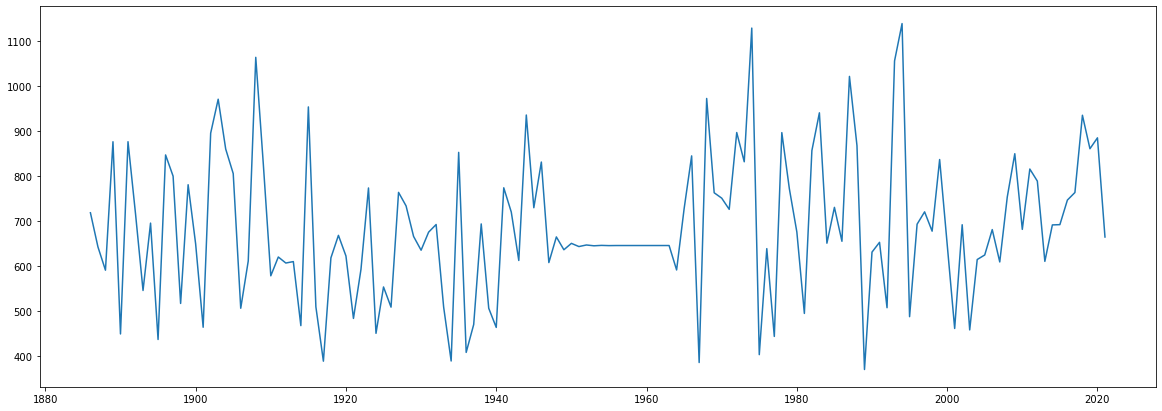
\includegraphics[scale=0.45]{images/line.png}
\caption{Biểu đồ đường}
\end{figure}

\begin{figure}[H]
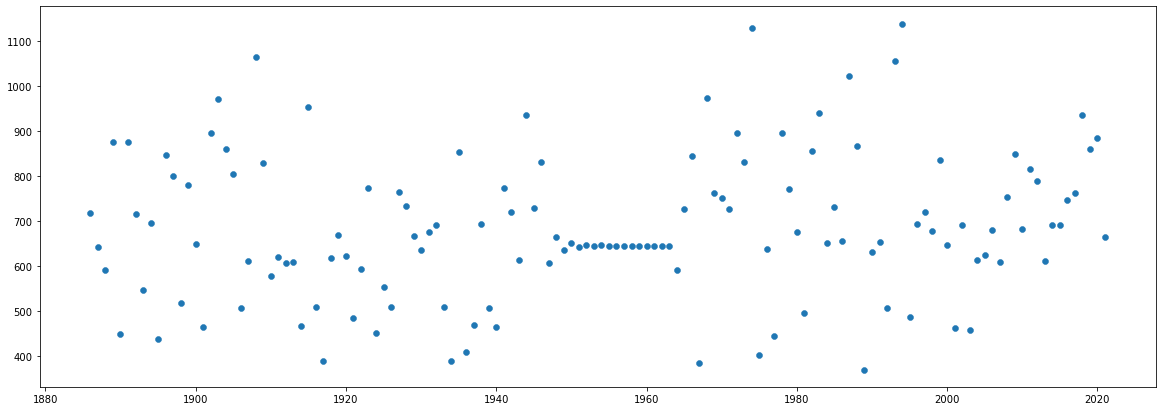
\includegraphics[scale=0.45]{images/scatterplot.png}
\caption{Biểu đồ phân tán}
\end{figure}

\end{center}
Sau đây là kết quả tính toán mode và median của dữ liệu.
\begin{center}
\begin{figure}[H]
\center{
\includegraphics[scale=1.5]{images/mode.png}}
\caption{Giá trị mode}
\end{figure}

\begin{figure}[H]
\center{
\includegraphics[scale=1.5]{images/median.png}}
\caption{Giá trị median}
\end{figure}

\begin{figure}[H]
\center{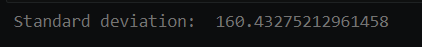
\includegraphics[scale=1.5]{images/sd.png}}
\caption{Giá trị độ lệch chuẩn}
\end{figure}
\end{center}
\subsection{Mô tả từ dữ liệu}
Ngoại trừ khoảng thời gian số liệu bị khuyết (số liệu của 14 năm, từ năm 1949 đến 1962), đã được tiền xử lý như trình bày trong phần trên, nhìn chung giá trị lượng mưa trung bình năm ở trạm Concordia Muni AP, Kansas, miền Tây Hoa Kỳ có sự biến động liên tục qua từng năm với những khoảng biến động tương ứng tương đối lớn (trên 300 mm) trong trung bình 2 lần trong 20 năm liên tiếp. 

Lượng mưa tại trạm này được tính trung bình trong khoảng 684.3 mm. Con số là xấp xỉ so với lượng mưa trung bình năm 2017 của Hoa Kỳ là 715mm (số liệu từ \url{https://en.wikipedia.org/wiki/List_of_countries_by_average_annual_precipitation}). Độ lệch chuẩn của dữ liệu lớn, dữ liệu phân bố không đều, có những năm lượng mưa đạt hơn 1100 mm, nhưng có những năm chỉ đạt ít hơn 400mm. Lượng mưa trung bình mỗi năm ở trạm này trong khoảng thời gian 1886 đến 2021 là lớn hơn 350 mm, chứng tỏ vùng đất này không bị hạn hán triền miên.\\
Có thể thấy, mặc dù trạm này không bị hạn hán triền miên, nhưng lượng mưa phân bổ không đều, có thể gây ảnh hưởng nghiêm trọng đến các hoạt động sản xuất, sinh hoạt của người dân nơi đây. Chính phủ sở tại cần đưa ra giải pháp nhằm giải quyết vấn đề này.

\newpage

\section*{Lời cảm ơn}
Trong quá trình thực hiện đồ án này, chúng em đã nhận được những bài giảng tận tâm, chi tiết về các phương pháp của Thầy Nguyễn Đình Thúc. Bên cạnh đó là những sự hướng dẫn của các Thầy, Cô trợ giảng cho môn học Toán ứng dụng và thống kê. Chúng em xin cảm ơn các Thầy, Cô.\\
Ngoài ra, chúng em cũng xin cảm ơn các bạn trong lớp đã đưa ra những chỉ dẫn, góp ý trong quá trình chúng em thực hiện đồ án.
\begin{flushright}
Thành phố Hồ Chí Minh, tháng 4 năm 2022
\end{flushright} 
\end{document}